\documentclass[a4paper,10pt,oneside,twocolumn,notitlepage,final]{jarticle}
\usepackage{ss15(UTF-8)}
\usepackage[dvipdfmx]{graphicx}
\usepackage{amsmath, caption, url, comment, here}
\usepackage{at-latex}
\captionsetup[figure]{font=small}

\author{谷口 暁星 (東京大学大学院 理学系研究科 天文学専攻 D1)}
\title{FMLO: オフ点不要の新しいミリ波サブミリ波分光法の開発と性能評価}

\begin{document}

\abst{
我々は, ヘテロダイン受信機の局部発振器 (Local Oscillator; LO)の発信周波数を変調 (Frequency Modulation; FM)することで単一鏡分光観測の感度を向上させる, 新しいミリ波サブミリ波分光法``FMLO''の開発を行っている。
本手法では従来のポジションスイッチ観測や周波数スイッチ観測で取得すべきオフ点 (参照スペクトル)の観測が不要なため, 観測効率の大幅な改善による感度の向上が可能である。
これは, 分光計出力を高頻度 ($\sim 10 \,\mathrm{Hz}$)で取得しつつ, LO周波数を変調させて天体信号を時間空間上で高周波に変調することにより, 低周波成分が卓越した$1/f$状の相関雑音と天体信号とを時系列データ上で分離することで実現している。
これにより, 観測効率および感度の向上とともに, ベースラインののうねりの低減, サイドバンドの分離が可能となり, 線幅の広い系外銀河の輝線探査やオフ点観測が難しい銀河面サーベイなどに, 絶大な威力が発揮されることが期待される。
本講演ではFMLOの原理に加え, 正確かつ高速な相関雑音の分離を可能にする解析パイプラインの開発, 野辺山45mミリ波望遠鏡へ搭載されたFMLOによる系内分子雲Ori-KLの性能評価観測について紹介する。
解析パイプラインの開発では, 連続波多素子カメラの反復モデリングを応用するとともに, 相関雑音の分離に主成分分析 (PCA)に確率モデルを導入することで, 天体信号スペクトルの再現性を大幅に改善が可能となった。
また性能評価観測では, 周波数変調の速度と幅のパターン(FMP)を最適化, およびFMLOを併用したマッピング観測を試験し, オフ点不要な天体画像が取得できることを実証した。
}

\section{Introduction}
ミリ波サブミリ波の連続波観測によって初期宇宙のダストに隠された爆発的星形成銀河の候補天体がこれまでにない感度と効率でサーベイされつつある今日, 分子や原子の輝線観測によってこれらの赤方偏移を決定し, 銀河の形成進化の知見を得るという点でミリ波サブミリ波分光観測は重要な意味を持つ。
一般的に遠方銀河の輝線は線幅が広くかつ弱いため, 高感度かつ高効率の分光観測が求められるが, ALMAの威力を持ってしてもなお一定の時間を要する上に, 競争率の高いALMAで多数の銀河サンプル対して膨大な時間をかけた分光サーベイを行うことは必ずしも効率的とは言えない。
そのため大口径の単一鏡による高感度かつ高効率な分光観測が重要となるが, 現在の一般的な分光観測手法であるポジションスイッチ法は目的天体 (オン点)に加え大気放射等の差し引きのために参照スペクトル (オフ点)の観測も交互に行う必要があるなど, 原理的に観測効率が低いという問題がある。
ポジションスイッチ法における感度$\Delta T$は以下の通りに表される。
ここで$T\msb{sys}$は大気込みのシステム雑音温度, $\Delta\nu$は分光計の周波数分解能, $t\msb{total}$は総観測時間, $\eta\msb{obs}$が総観測時間に対するオン点観測時間の割合 (観測効率)となる。
\begin{equation}
    \Delta T
    \simeq\frac{\sqrt{2}\,T\msb{sys}}{\sqrt{\Delta\nu\, t\msb{total}\, \eta\msb{obs}}}
    =\frac{\sqrt{2}\,T\msb{sys}}{\sqrt{\Delta\nu\, t\msb{ON}}}
    \label{noiselevel}
\end{equation}
高赤方偏移天体のように頻繁にオフ点を観測する必要がある場合や, 銀河面サーベイのように至る所に輝線が存在するためオフ点をオン点の近くに取れない場合は観測効率が特に低くなり, 実効的な感度の悪化につながる。

\vspace{2mm}
\begin{minipage}{0.2\textwidth}
    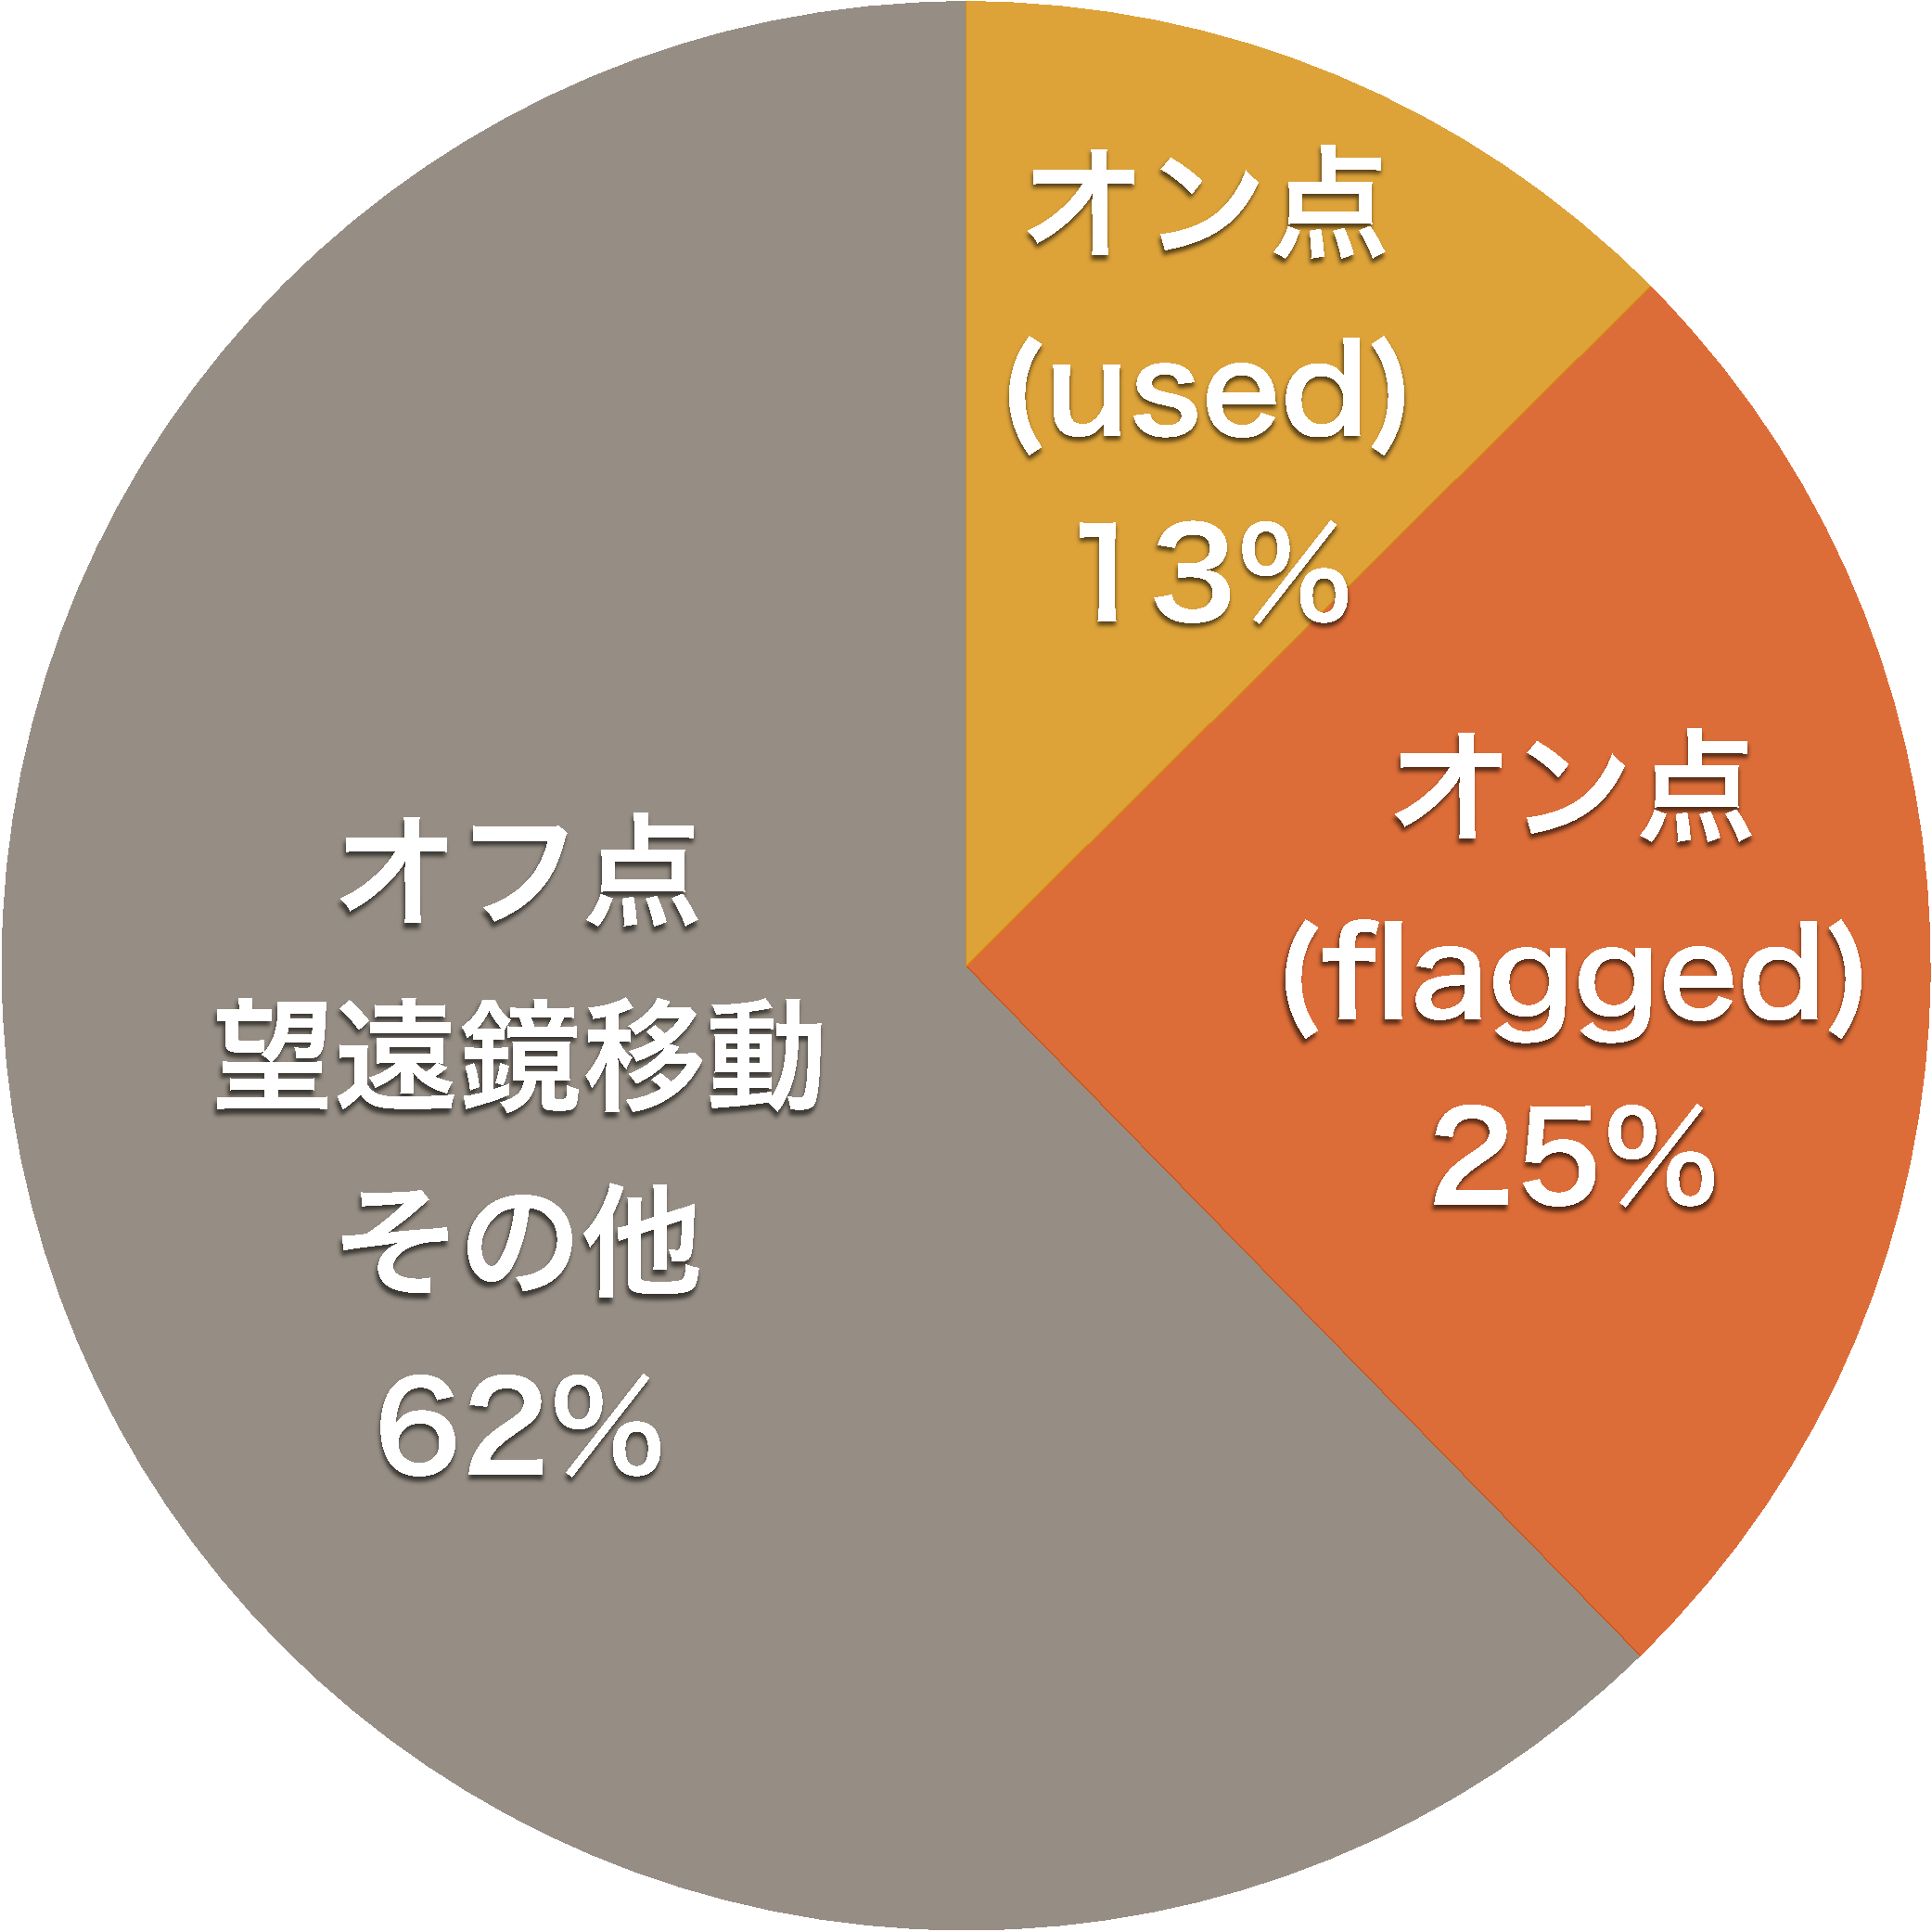
\includegraphics[width=\textwidth]{fig/obstime.pdf}
\end{minipage}
\hfill
\begin{minipage}{0.23\textwidth}
    \small{図1: 野辺山45m望遠鏡での高赤方偏移天体の分光観測の観測時間の内訳。オン点の割合はフラグ分も合わせても4割未満であり, 実効的に感度を2倍程度悪化させることに相当する。}
\end{minipage}
\vspace{2mm}
\setcounter{figure}{1}
\begin{figure*}[!t]
    \centering
    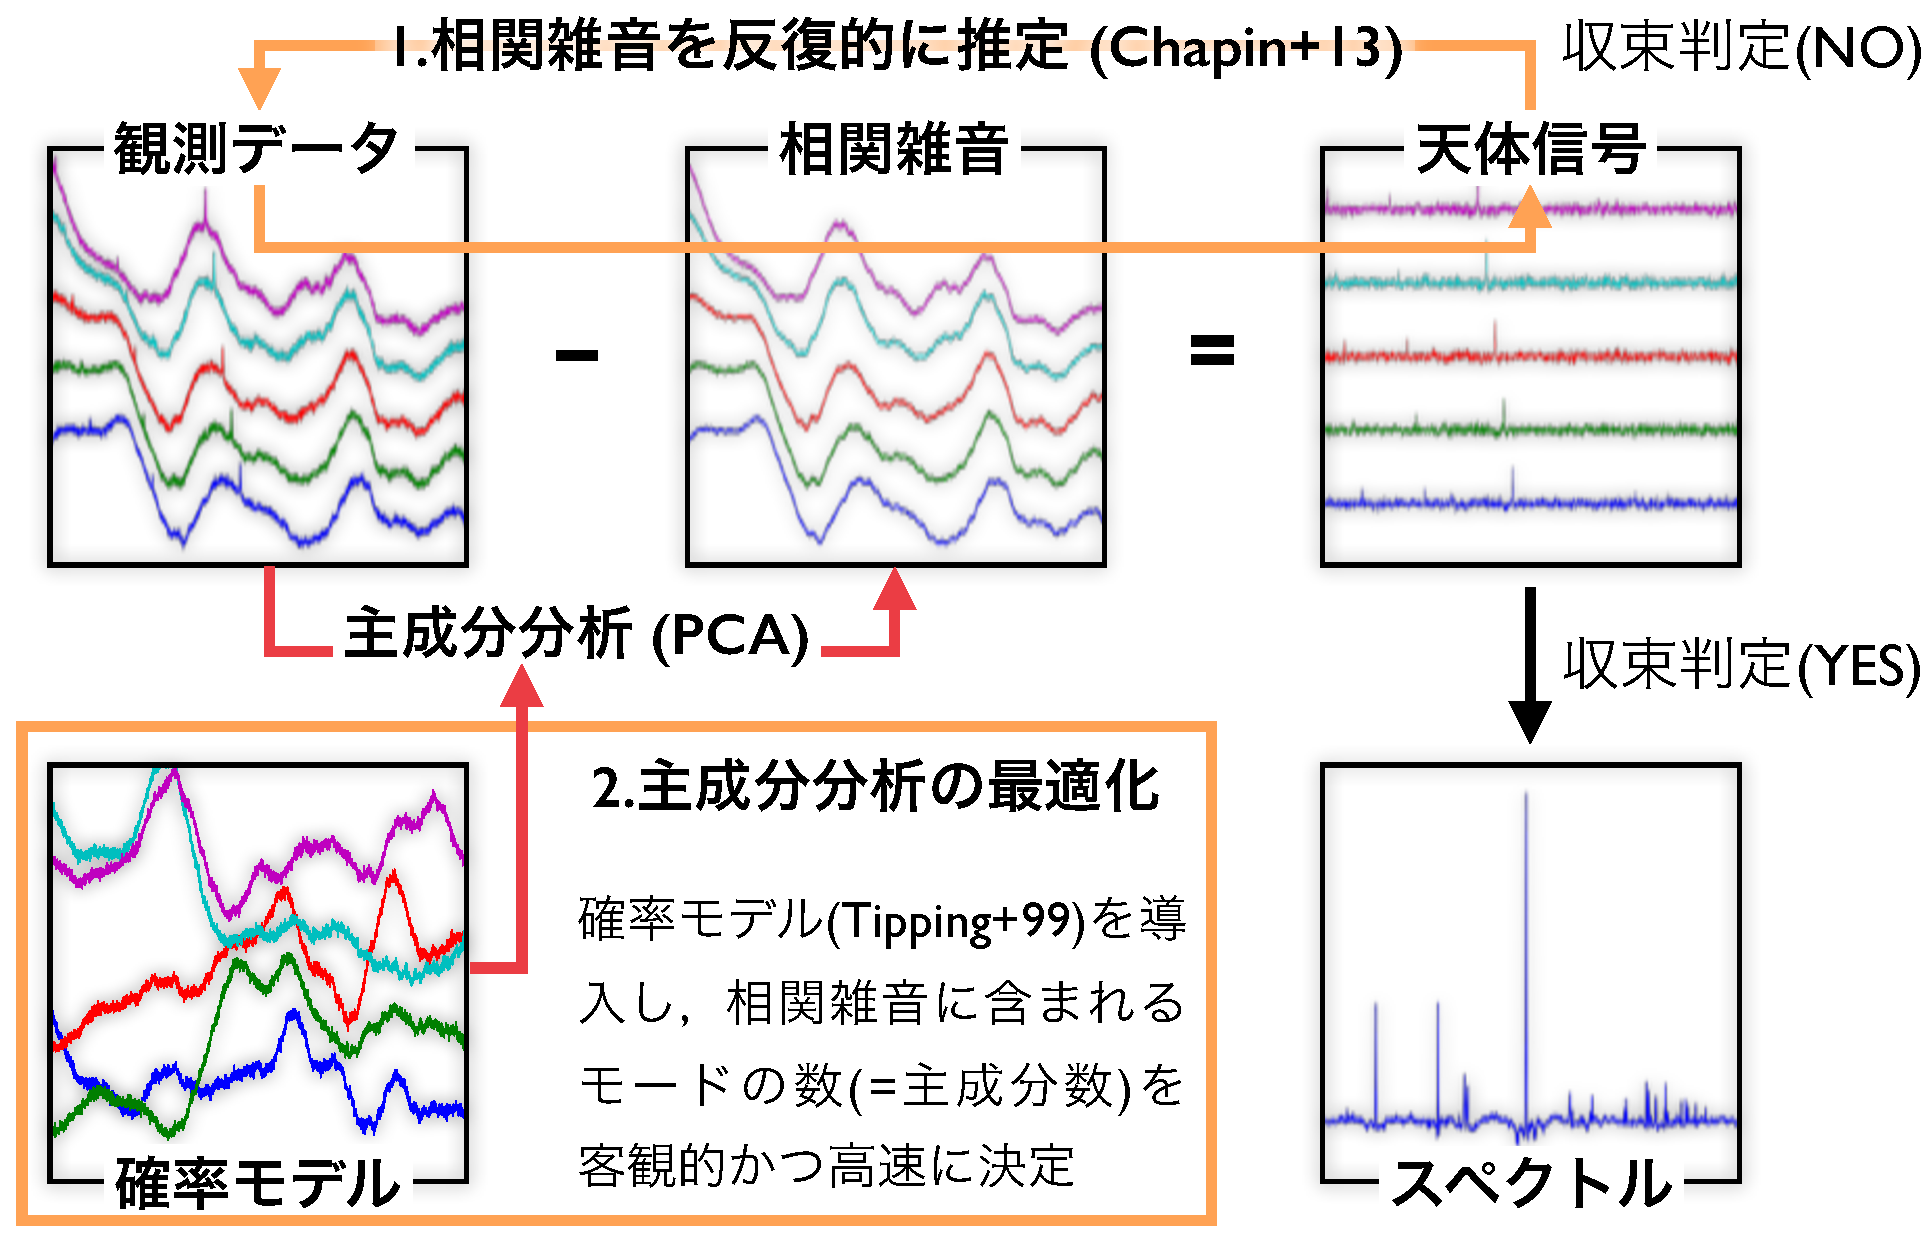
\includegraphics[width=0.8\textwidth]{fig/fmlo.pdf}
    \caption{FMLO法の原理と本研究で導入された2つのデータリダクション手法の概念図。$10\uni{Hz}$で取得される観測データ (分光計サンプル)はFMLOによって天体信号が入射するチャンネルが次々と変化している様子が分かる。これらの時系列データから主成分分析 (PCA)によって相関雑音を推定することにより, 天体信号との分離が可能となる。本研究では相関雑音を反復的に推定し, さらに各推定の際に確率モデルを用いた主成分分析の最適化を行うことで, 輝線のプロファイルの再現性を大幅に改善することに成功した。}
    \label{fmlo}
\end{figure*}

また, ポジションスイッチ法ではオン点からオフ点を差し引く際にスペクトルのベースラインがうねることがある。
これは強度が小さい高赤方偏移天体の分光観測において大きな問題であり, たとえ長時間積分によって感度を$1/\sqrt{t\msb{ON}}$に従って改善できたとしても,
感度に対してうねりが大きく残ってしまうことにより輝線が埋もれてしまい, 検出できない可能性がある。
以上より, 従来のポジションスイッチ法における問題点を解決し, 感度と観測効率の向上させるような観測手法が必要となるのである。

\vspace{-5mm}
\section{Principle}
そこで, 周波数変調局部発振器(Frequency Modulation Local Oscillator; \textbf{FMLO})による, オフ点の観測を必要としない新しい単一鏡分光手法 (Tamura et al. 2013)に注目した。
これは, 連続波多素子カメラの分野で多大な成果を収めている, カメラの素子に同時に降り注ぐ相関雑音の分離という考え方を分光観測に応用したものである。
すなわち, \textbf{局部発振器(LO)の周波数を変調(FM)させることで天体信号が入射するチャンネルを次々と変化させながら, 分光計出力を高頻度 (10 Hz)に取得することで, 時系列データ上で分光計チャンネルに同時に降り注ぐ相関雑音の分離を達成する観測手法}である。
FMLO法の原理は\figref{fmlo}に示されている。
ヘテロダイン受信機に入力されるLO信号は, ポジションスイッチ法では観測を通して一定の周波数である。
一方, FMLO法では分光計サンプルごとにLO周波数が変調されるため, 天体信号は時間空間上で高周波数 (10 Hz)に変調される。
これに対し, 地球大気放射, 受信機の周波数特性などは低周波成分 ($<1\uni{Hz}$)が卓越した相関雑音として振る舞うため, 主成分分析 (PCA)を用いて天体信号との分離が可能になるのである。

FMLO法はオフ点の観測を必要としないため観測効率がほぼ100\%であり, 式\eqref{noiselevel}に従って感度の劇的な向上が可能となる。
また, 分光計サンプルごとに相関雑音が分離されるため, スペクトルのベースラインの安定性が大きく改善される。

しかし, 上記の手法では広がった構造を持ち強度の大きい輝線のプロファイルの再現性が悪いことが知られていた。
これは主成分分析の際に最適な主成分の数が決定できていないことに加え, 1回のみの相関雑音の推定では輝線が相関雑音から十分分離できていないことが原因であり, これの解決が課題となる。
\begin{figure*}[!ht]
    \centering
    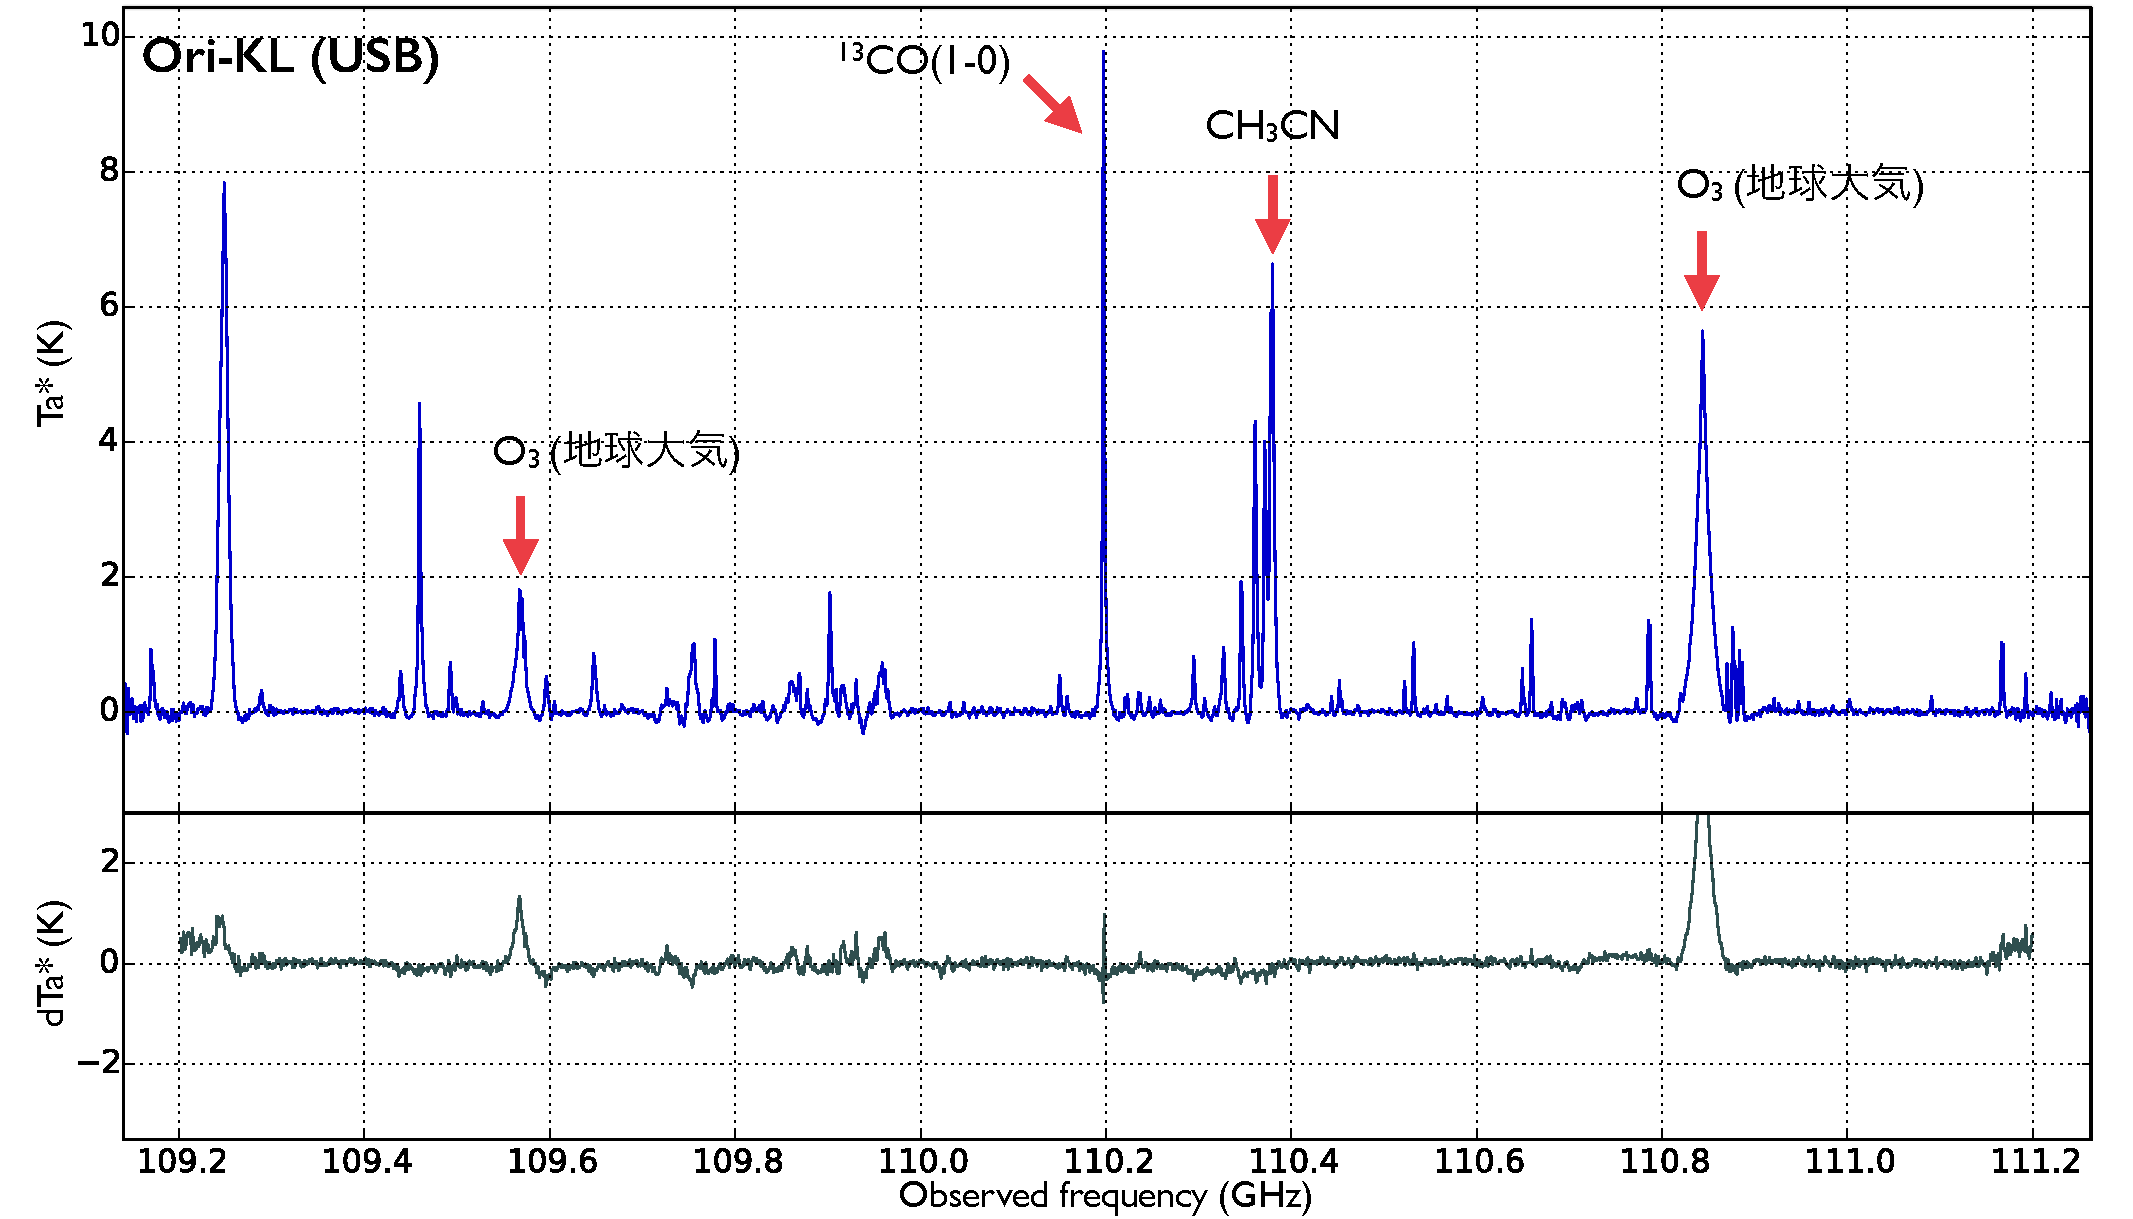
\includegraphics[width=0.8\textwidth]{fig/spec.pdf}
    \caption{系内分子雲Ori-KLを最適な変調パターンで観測し, 本研究で導入した2つのデータリダクション手法を用いて解析したスペクトル (上)と, 従来のポジションスイッチ法で観測されたスペクトルとの残差 (下)。FMLO法では地球大気由来の分子も検出されるため, この部分の残差は大きくなる。}
    \label{spec}
\end{figure*}

\section{Development}
そこで, 本研究では\figref{fmlo}に示した2つのデータリダクション手法を導入することで, 輝線のプロファイルの再現性を大幅に改善することに成功した。

\vspace{-5mm}
\subsection{相関雑音の反復的推定}
連続波多素子カメラにおいて用いられている, 相関雑音の反復的推定の手法 (Chapin et al. 2013)をFMLO法のデータリダクションに応用した。
この手法では, $n\,(\geq2)$回目の相関雑音の推定を, 観測データから$n-1$回目に推定された天体信号を予め引き去った上で行う。
これにより, 輝線の影響を最小限に抑えて相関雑音の推定が可能となる。

\vspace{-5mm}
\subsection{主成分分析の最適化}
相関雑音の推定に用いる主成分分析の主成分数は, その数が小さすぎると相関雑音の天体信号への漏れこみが大きくなり, ベースラインのうねりが生じる。
反対に大きすぎると天体信号まで相関雑音として推定することになるため, 輝線のプロファイルの再現性が悪化する。
そこで, 主成分分析に確率的な解釈を導入した確率的主成分分析 (PPCA)によるベイズ的な取り扱い (Minka et al. 2001)により,
最適な主成分数の客観的かつ高速な計算が可能となった。

実際にこの手法で正しい主成分数の推定ができていることを示したのが\figref{ppca}である。
最適な主成分数の計算方法の一つとして, 相関雑音の分離後の観測データにおける共分散成分の割合が最小となるように決めるという手法が考えられるが, PPCAによる計算は前者の最小値付近を正しく推定していることが確認できる。
膨大な計算量を必要とする前者に対し, 後者のPPCAは1--2桁程度小さい計算量で済むため, 反復的推定に組み込むことが可能である。
\begin{figure}[!hb]
    \centering
    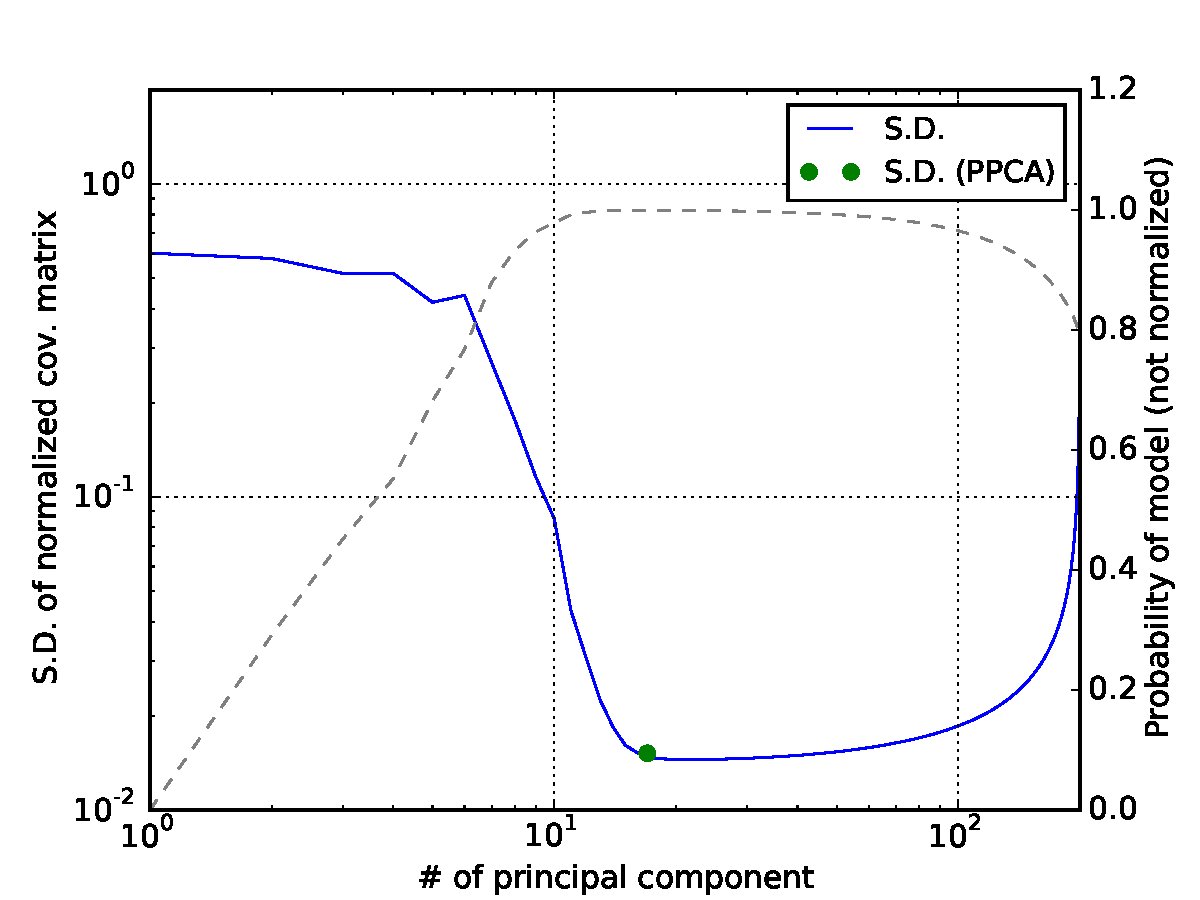
\includegraphics[width=0.4\textwidth, bb=0 0 576 400, clip]{fig/ppca_vs_conventional.pdf}
    \caption{主成分数を変化させたときの相関雑音分離後の観測データにおける共分散成分の割合 (青線)と, PPCAによって決定された主成分数 (緑点)。}
    \label{ppca}
\end{figure}
\begin{figure*}[!ht]
    \centering
    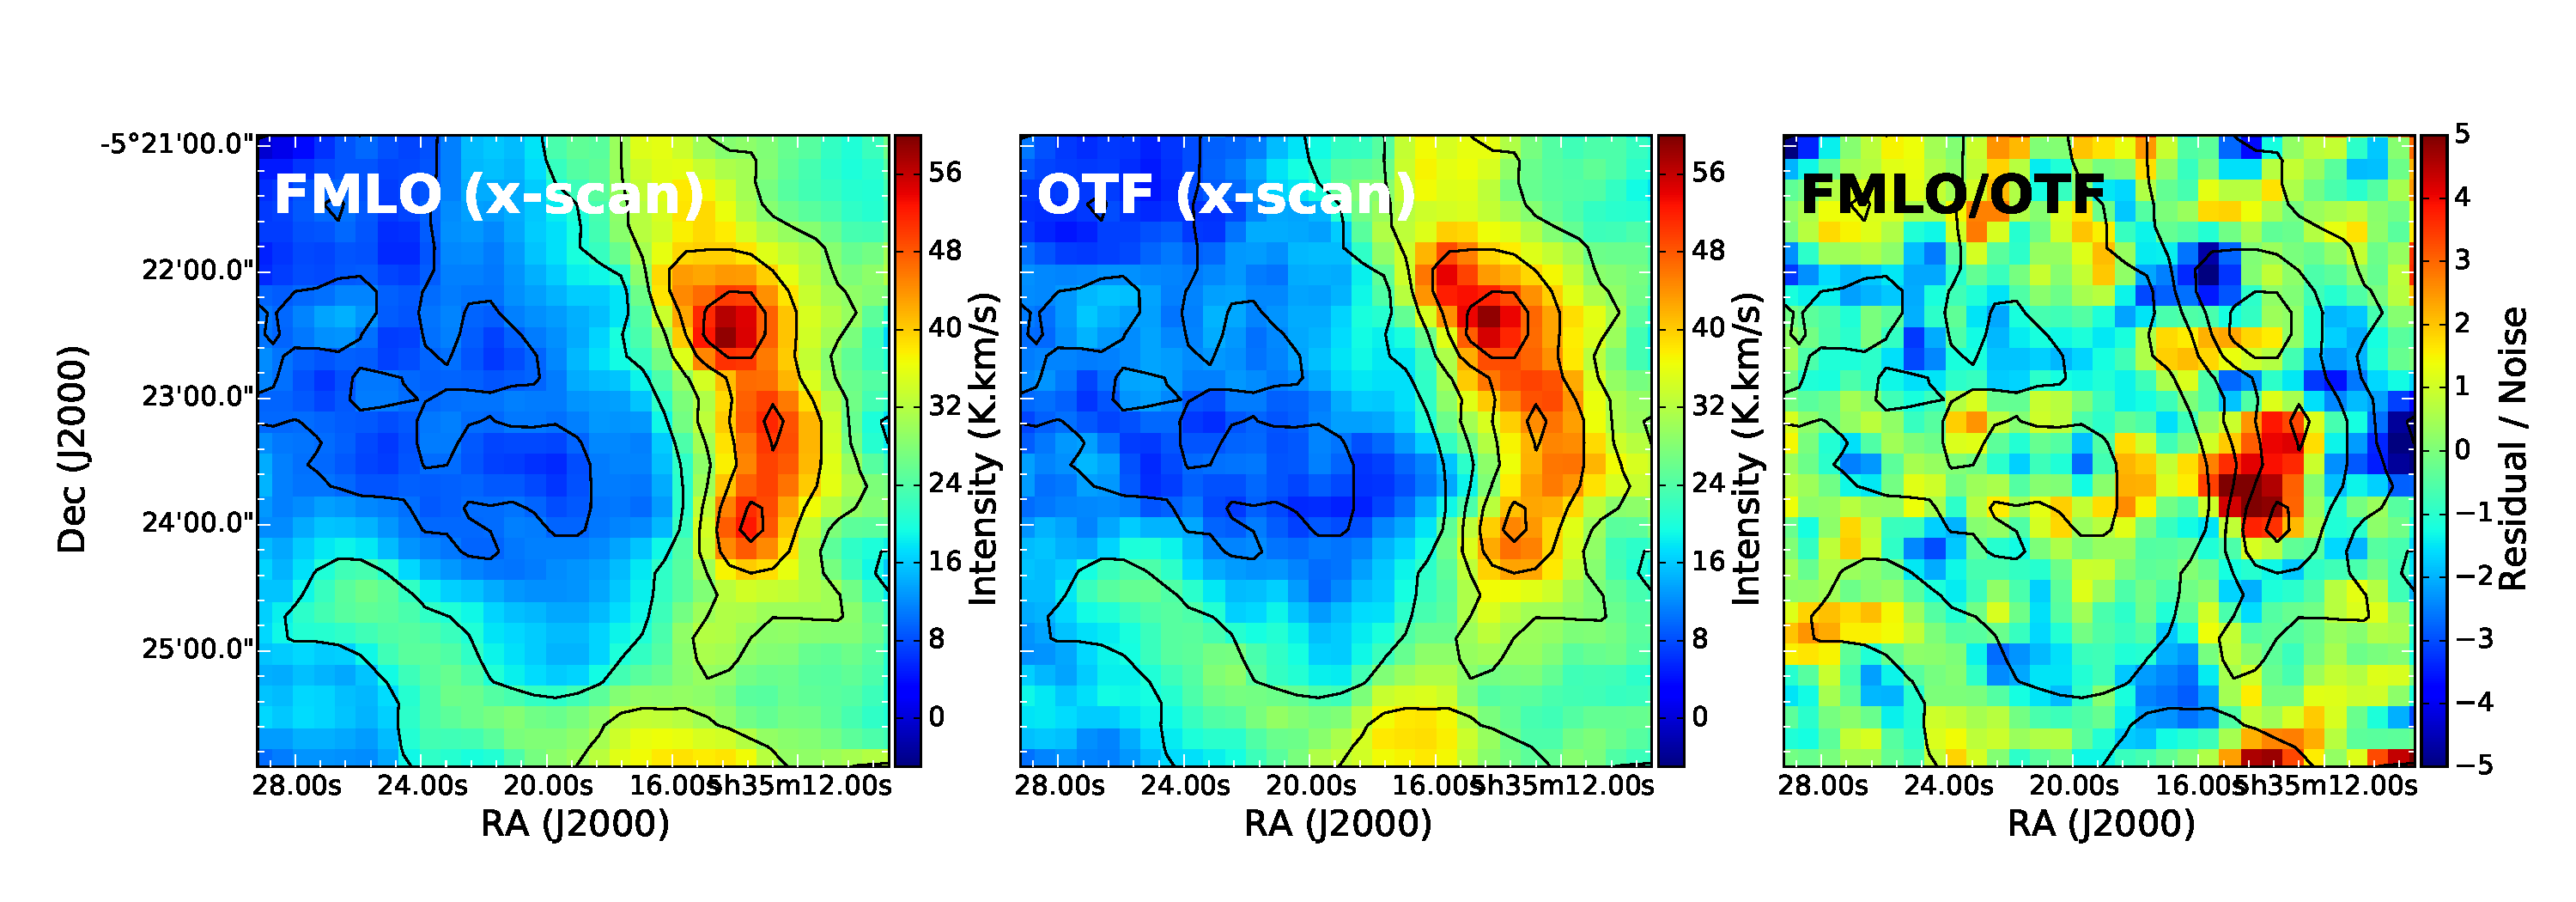
\includegraphics[width=0.9\textwidth]{fig/otf.pdf}
    \caption{系内分子雲Ori-KLの$^{13}$CO J=1-0をFMLOマッピング法で観測して得られた積分強度マップ (左), 従来のOTF観測で得られた積分強度マップ (中央), これらの残差のノイズレベルに対する割合を表すS/Nマップ (右)。}
    \label{otf}
\end{figure*}

\section{Observation \& Evaluation}
FMLO法の科学的立証のため, 野辺山45m望遠鏡に搭載されたFMLOを用いた試験観測が2014年に行われ, 本研究で導入されたデータリダクション手法を用いた性能評価が行われた。
ここでは紙面の都合上, 特に重要となる変調パターン最適化試験とFMLOマッピング試験について紹介する。

\vspace{-5mm}
\subsection{変調パターン最適化試験}
FMLO法ではLO周波数を変調させる際, 分光計サンプル間の変調ステップと変調幅を観測する輝線に対して最適化させる必要がある。
そこで試験観測ではこの2つを様々に変えた``変調パターン''を作成し, これを用いてFMLO法での観測を行った。
その結果, 輝線の半値幅より十分大きな変調ステップ, かつ観測バンドに対して大きく振りすぎない変調幅が最適な変調パターンであることが確認された。
最適な変調パターンで観測された系内分子雲Ori-KLのスペクトルを\figref{spec}に示した。
従来のポジションスイッチ法と比較して広がった構造や強度の大きい輝線のプロファイルが再現できることが示された。

\vspace{-5mm}
\subsection{FMLOマッピング試験}
FMLO法で観測を行いながら, 空間的にOTF (On-the-fly)観測を行うことで, オフ点の取得を必要としないFMLOマッピング観測の実証試験を行った。
性能評価では, 主成分分析による天体信号の推定に加え, スペクトルの空間情報も利用することでより正確な天体信号の推定が可能となるようデータリダクションを行っている。
同様にOri-KLを観測し, 取得した$^{13}$COの積分強度マップを\figref{otf}に示した。
その結果, FMLOマッピング観測は従来のポジションスイッチ法を用いたOTF観測を十分再現でき, FMLO法のマッピングへの応用が実証された。

\vspace{-5mm}
\section{Conclusion \& Future Plans}
本研究\footnote{本集録の内容を含む研究内容全体は谷口の修士論文としてまとめられ, \url{http://www.ioa.s.u-tokyo.ac.jp/~taniguchi/#!fmlo/downloads.md}にPDFが公開されている。}
によってFMLO法のデータリダクション手法が確立され, 試験観測と性能評価によって従来の観測と矛盾ないスペクトルやマップが取得できることが確認された。
FMLOは新しいミリ波サブミリ波分光法として, 大阪府立大1.85m望遠鏡, 中米LMT, 計画中のLST50m望遠鏡などの大口径の単一鏡への搭載, 検討が進んでいるところである。

\vspace{-5mm}
\section*{Acknowledgement}
\noindent
本研究は新学術領域研究``重力波天体の多様な観測による宇宙物理学の新展開''のサポートを受けています。
また基礎物理学研究所 (研究会番号:YITP-W-15-04)および国立天文台のご支援に感謝いたします。

\vspace{-5mm}
\section*{Reference}
\noindent
$\bullet$ Y. Tamura et al. 2013, ASPCS, 476, 401\\
$\bullet$ E. L. Chapin et al. 2013, MNRAS, 430, 2545\\
$\bullet$ T. P. Minka et al. 2000, NIPS, 15, 598
\vspace{5mm}
\end{document}
